\documentclass[conference]{IEEEtran}
\IEEEoverridecommandlockouts
\usepackage{cite}
\usepackage{amsmath,amssymb,amsfonts}
\usepackage{algorithm}
\usepackage{algorithmic}
\usepackage{graphicx}
\usepackage{textcomp}
\usepackage{booktabs}
\usepackage{xcolor}
\usepackage{tikz}
\usetikzlibrary{shapes.geometric,arrows.meta,positioning,calc}
\def\BibTeX{{\rm B\kern-.05em{\sc i\kern-.025em b}\kern-.08em
    T\kern-.1667em\lower.7ex\hbox{E}\kern-.125emX}}

%% abstract, index terms and section lead-ins run at normal weight
\makeatletter
\def\@IEEEabskeysecsize{\normalsize\normalfont}
\makeatother

%% tighter float separation to hold the 6-page limit
\setlength{\textfloatsep}{9pt plus 2pt minus 2pt}
\setlength{\dbltextfloatsep}{9pt plus 2pt minus 2pt}
\setlength{\floatsep}{7pt plus 2pt minus 2pt}
\setlength{\dblfloatsep}{7pt plus 2pt minus 2pt}
\setlength{\abovecaptionskip}{3pt}
\setlength{\belowcaptionskip}{0pt}

\begin{document}

\title{A Dual-Task Deep Learning Framework for\\
Multi-Label Thoracic Pathology Classification\\
and Spatial Localization in Chest Radiographs\\
with Grad-CAM Explainability}

%% Five authors, each with their own affiliation block, arranged 3 + 2.
%% IEEEtran's \and mechanism cannot fit five columns at this affiliation width,
%% so the two rows are laid out in a tabular.
\newcommand{\authcell}[3]{%
  \parbox[t]{#1}{\centering #2\\[0.3ex]
  {\small\textit{Dept. of Electronics \&}\\
  \textit{Communication Engineering}\\
  \textit{PES University}\\
  Bangalore, India\\
  #3}}}

\author{%
\begin{tabular}{@{}c@{\hspace{2mm}}c@{\hspace{2mm}}c@{}}
\authcell{0.315\textwidth}{Allan Suraj}{allansuraj4821@gmail.com} &
\authcell{0.315\textwidth}{Anish Ganesh}{anishganesh2004@gmail.com} &
\authcell{0.315\textwidth}{Arpan Murthy}{arpan07murthy@gmail.com} \\
\noalign{\vskip 3.2ex}
\multicolumn{3}{c}{%
  \authcell{0.345\textwidth}{Kshitij Narendrakumar Nagashetti}{kshitijnarendrakumar@gmail.com}%
  \hspace{10mm}%
  \authcell{0.345\textwidth}{Rashmi N Ugarakhod}{rashmin@pes.edu}}
\end{tabular}
}

\maketitle

\begin{abstract}
\normalfont
No imaging study is ordered more often than the chest film, and few are harder
to automate well. Reading one is slow, two readers do not always agree, and the
answer is rarely a single label, since one film commonly carries several
findings at once. Published systems tend to solve either the whole-image
labelling problem or the region-finding problem, and seldom expose why a
prediction was made in a form a clinician could check. This paper presents a dual-task framework that couples (i) multi-label
pathology classification on MIMIC-CXR using a DenseNet-121 backbone trained
with binary Focal Loss ($\alpha{=}0.25$, $\gamma{=}2.0$) to address the
negative-to-positive label skew typical of medical corpora, and (ii) pathology
localization on the radiologist-annotated VinDr-CXR dataset using a Faster
R-CNN detector riding on an FPN neck. Grad-CAM is read off the
final dense block to generate saliency maps for high-confidence predictions,
and checkpoint weight averaging over disjoint patient subsets is used to
stabilize generalization. Training uses Adam with ReduceLROnPlateau scheduling
and mixed precision, which improved throughput by up to $2.5\times$. The
classifier achieves a micro F1 of 0.7528 at under 25\,ms per image on a single
CUDA GPU. On a 498-image patient-disjoint validation subset the mean AUC-ROC is
0.759, below the range reported in the literature. The per-class breakdown is
given: ranking remains strong for
large findings (0.87 for cardiomegaly and lung opacity) but approaches chance
for small focal ones (0.54 for pneumothorax), and top-1 predictions concentrate
on five of fourteen categories. The system is deployed as an interactive
Streamlit application (MED-AI Visualizer) showing the raw radiograph, the
predicted boxes and the saliency heatmap together. The training protocol, the
observed failure modes and a corrective plan are described.
\end{abstract}

\begin{IEEEkeywords}
\normalfont
chest radiography, multi-label classification, object detection, Faster R-CNN,
DenseNet, focal loss, class imbalance, explainable artificial intelligence,
Grad-CAM, MIMIC-CXR, VinDr-CXR, computer-aided diagnosis
\end{IEEEkeywords}

\section{Introduction}

A large fraction of the diagnostic imaging performed anywhere in the world is
plain chest radiography (CXR). It is cheap, quick, delivers little dose, and can
be had in places where CT or MR cannot, which is why it remains the opening
examination whenever pulmonary, pleural or cardiac disease is suspected. Sheer
volume brings its own problems. Reporting queues build up, and how well a film
is read depends on who is reading it, how tired they are and how awkward the
case is. Software that could order a worklist by urgency, surface the findings
that will not wait, and show what it based that on would therefore be of real
use.

Three properties make CXR interpretation harder than the natural-image
benchmarks on which modern convolutional networks were developed.

First, one film can carry many labels at once, so this is not a choice among
alternatives. Cardiomegaly, pulmonary edema and bilateral effusion may all appear
together in congestive heart failure. Treating the classes as mutually exclusive,
which a softmax head does, is wrong here. Independent per-class sigmoids
are required instead, and this choice affects the loss function, the
thresholding strategy and the evaluation metrics.

Second, label distributions are heavily skewed. Pneumothorax, rib fracture and
lung lesion each occur in well under 5\% of studies. Under binary cross-entropy
the gradient is dominated by easy negatives, and the optimizer tends to
converge to a degenerate solution that predicts ``absent'' for every rare
pathology while still recording a low training loss.

Third, a label on its own is of limited clinical use. A radiologist acting on
an automated finding needs to know where the supporting evidence lies, both as
coarse attention and as a box that can be measured against normal ranges.

All three are handled inside one deployable pipeline: an independent-sigmoid
head for the label space, Focal Loss re-weighting for the skew, and, for the
evidence, Grad-CAM saliency read off the classification backbone alongside a
detector trained separately on radiologist-drawn boxes.

\textit{Contributions.} (1) A dual-task, dual-dataset framework that provides
image-level diagnosis (MIMIC-CXR, 14 CheXpert-derived pathologies) and
region-level localization (VinDr-CXR) behind a single inference interface,
despite the disjoint label taxonomies. (2) A focal-loss imbalance treatment
specified in sufficient detail for reproduction, covering the $\alpha/\gamma$
parameterization, the optimizer schedule and the mixed-precision engine. (3) A
patient-disjoint training and checkpoint-averaging protocol with no identity
leakage between splits. (4) An explainability layer that combines Grad-CAM
saliency with detector boxes at inference time. (5) A clinician-facing
deployment with runtime backbone switching at sub-25\,ms inference. (6) A report that includes a negative
finding, its probable cause and the remedy.

\section{Related Work}

Learning at scale on thoracic films became tractable once ChestX-ray14
\cite{wang2017} released 112,120 frontal studies whose labels had been recovered
automatically from their reports. CheXNet \cite{rajpurkar2017} built on that
release with a 121-layer DenseNet reported to out-rank practising radiologists
on pneumonia. The labelling scheme itself was sharpened by CheXpert
\cite{irvin2019}, which handled uncertainty explicitly and fixed a vocabulary
that MIMIC-CXR-JPG \cite{johnson2019jpg} subsequently adopted. Baltruschat
\textit{et al.} \cite{baltruschat2019} reported that backbone choice matters
less than input resolution and the handling of label noise, which is why the
present work concentrates on loss design rather than on a backbone search.
Majkowska \textit{et al.} \cite{majkowska2020} argued for
radiologist-adjudicated reference standards.

Whole-image labels say nothing about location. VinDr-CXR \cite{nguyen2022}
closes that gap: seventeen radiologists marked 18,000 films, three of them per
training study and five in consensus per test study, yielding an unusually
dependable spatial ground truth.
Detection is still dominated by two-stage Faster R-CNN \cite{ren2015}, and the
Feature Pyramid Network \cite{lin2017fpn} supplies the multi-scale semantics
needed here, since lesion diameters on a chest film vary over two orders of
magnitude. Backbone choice trades accuracy against latency, with ResNet-50
\cite{he2016} offering capacity and MobileNetV3-Large \cite{howard2019}
real-time inference on modest hardware. Ensembling requires box-level
fusion, for which greedy NMS and weighted box fusion \cite{solovyev2021} are
standard.

Focal Loss \cite{lin2017focal} was introduced to prevent dense detectors from
being overwhelmed by background anchors, down-weighting well-classified
examples through a $(1-p_t)^\gamma$ factor. Its transfer to multi-label medical
classification is straightforward, since each independent binary problem
exhibits the same easy-negative dominance. Grad-CAM \cite{selvaraju2017}
weights feature maps by gradients of the class score, which makes saliency
available from any CNN. Saliency is not a substitute for localization
supervision, since it produces only coarse class-discriminative attention. For
this reason a separately supervised detector is retained here rather than
treating a heatmap as a proxy for a box. Most existing systems address a single
aspect of the problem: one benchmark, detection alone, or an explanation module
added to a fixed classifier. The framework below combines these components in one
pipeline.

\begin{figure*}[!t]
\centering
\scriptsize
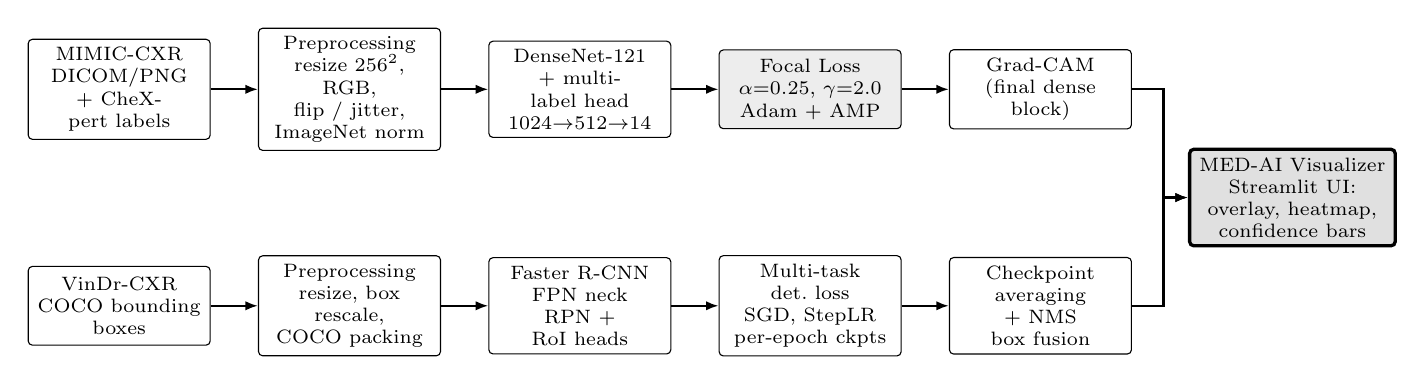
\begin{tikzpicture}[
  node distance=6mm and 6mm,
  box/.style={draw, rounded corners=1.5pt, align=center, inner sep=3pt,
              minimum height=10mm, text width=21mm, font=\scriptsize},
  shaded/.style={box, fill=black!7},
  final/.style={box, fill=black!12, very thick, text width=24mm},
  ar/.style={-{Latex[length=1.6mm]}, thick}
]
\node[box] (m1) {MIMIC-CXR\\ DICOM/PNG\\ + CheXpert labels};
\node[box, right=of m1] (m2) {Preprocessing\\ resize $256^2$, RGB,\\ flip / jitter,\\ ImageNet norm};
\node[box, right=of m2] (m3) {DenseNet-121\\ + multi-label head\\ $1024{\to}512{\to}14$};
\node[shaded, right=of m3] (m4) {Focal Loss\\ $\alpha{=}0.25$, $\gamma{=}2.0$\\ Adam + AMP};
\node[box, right=of m4] (m5) {Grad-CAM\\ (final dense block)};

\node[box, below=16mm of m1] (v1) {VinDr-CXR\\ COCO bounding\\ boxes};
\node[box, right=of v1] (v2) {Preprocessing\\ resize, box rescale,\\ COCO packing};
\node[box, right=of v2] (v3) {Faster R-CNN\\ FPN neck\\ RPN + RoI heads};
\node[box, right=of v3] (v4) {Multi-task det.\ loss\\ SGD, StepLR\\ per-epoch ckpts};
\node[box, right=of v4] (v5) {Checkpoint\\ averaging\\ + NMS box fusion};

\node[final] at ($(m5)!0.5!(v5) + (32mm,0)$) (ui)
  {MED-AI Visualizer\\ Streamlit UI:\\ overlay, heatmap,\\ confidence bars};

\draw[ar] (m1) -- (m2); \draw[ar] (m2) -- (m3); \draw[ar] (m3) -- (m4);
\draw[ar] (m4) -- (m5);
\draw[ar] (v1) -- (v2); \draw[ar] (v2) -- (v3); \draw[ar] (v3) -- (v4);
\draw[ar] (v4) -- (v5);
\draw[ar] (m5.east) -- ++(4mm,0) |- (ui.west);
\draw[ar] (v5.east) -- ++(4mm,0) |- (ui.west);
\end{tikzpicture}
\caption{End-to-end architecture. The upper path performs image-level
multi-label diagnosis with a Focal-Loss-trained DenseNet-121 and a Grad-CAM
explanation. The lower path performs radiologist-supervised bounding-box
localization with Faster R-CNN/FPN. Both paths converge in the deployed MED-AI
Visualizer.}
\label{fig:arch}
\end{figure*}

\section{Methodology}

\subsection{Datasets and working taxonomy}

The image-level branch draws on MIMIC-CXR \cite{johnson2019mimic}, a corpus of
de-identified thoracic films paired with the text of their radiology reports.
Supervision comes from its JPG release \cite{johnson2019jpg}, in which fourteen
observation flags per study are recovered automatically from the report text
under the CheXpert labelling scheme \cite{irvin2019}. Studies are filed by
patient prefix, and the experiments here draw on prefixes p13 through p19.

Region-level supervision comes from VinDr-CXR \cite{nguyen2022}, which
contributes 18,000 postero-anterior films divided 15,000 for training and 3,000
for testing. Annotations ship as one CSV row per reader; we re-serialized them
into COCO-style JSON, rewrote every box as $[x_{\min}, y_{\min}, w, h]$ and
reserved a background index. The reader vocabulary was collapsed to the fifteen
thoracic finding classes kept for detection.

Both branches report against one shared 14-class label space, used throughout
Section~\ref{sec:results} and by the deployed system; its members are the row and
column headings of Fig.~\ref{fig:cm}. Against the native
VinDr list this folds nodule together with mass and puts interstitial lung
disease and lung opacity in place of the two fracture classes. We release the
mapping alongside the code.

\subsection{Preprocessing and patient-disjoint splits}

One front-end serves both corpora and accepts either as input. Each film is
rescaled to $256 \times 256$ and its single grey channel replicated three times,
which lets pretrained ImageNet filters be loaded without touching the stem
convolution. Augmentation during training is limited to
\texttt{RandomHorizontalFlip()} and \texttt{ColorJitter(0.1, 0.1)}; the jitter
is deliberately weak, since absolute grey level on a radiograph is itself
diagnostic. Normalization uses the channel means $(0.485, 0.456, 0.406)$ and
deviations $(0.229, 0.224, 0.225)$ that ship with the pretrained weights. Partitioning
happens at the patient-prefix level, which keeps any single patient out of both
the training and the validation half and so avoids the identity leakage that
otherwise flatters reported CXR numbers. As a sanity check the parsed boxes
were painted back onto their films and a sample compared against the reader
annotations, exposing a coordinate-convention error and a scaling error that
the loss curve gave no sign of.

\subsection{Framework overview}

Fig.~\ref{fig:arch} summarizes the pipeline. The two branches share a
preprocessing front-end and a visualization back-end. The classification branch
produces 14 independent pathology probabilities and, for every prediction above
the display threshold, a Grad-CAM saliency map. The localization branch
produces scored bounding boxes. A fusion stage merges evidence across
checkpoints and renders the composite result.

\subsection{Classification branch and Focal Loss}

The classifier is built on DenseNet-121 \cite{huang2017}. Each layer inside a
dense block takes as input every earlier activation stacked along channels,
$x_\ell = H_\ell([x_0, \ldots, x_{\ell-1}])$, with $H_\ell(\cdot)$ standing for
the batch-norm, ReLU and convolution composite. Because features are reused
rather than discarded, fine texture survives to the top of the network:
reticular patterns, small nodular opacities and faint pleural lines are exactly
the cues fine-grained radiographic reading turns on. Weights are initialized
from ImageNet \cite{deng2009} and the 1000-way head swapped for
\begin{equation}
\hat{y} = \sigma\!\left(W_2 \,\mathrm{Drop}_{0.2}(\mathrm{ReLU}(W_1 f))\right),
\end{equation}
with $f \in \mathbb{R}^{1024}$ the globally pooled feature vector, $W_1 \in
\mathbb{R}^{512 \times 1024}$, $W_2 \in \mathbb{R}^{14 \times 512}$ and
$\sigma(\cdot)$ the element-wise sigmoid. Using $C = 14$ independent sigmoids
rather than a softmax allows co-occurring pathologies to be predicted
simultaneously.

Write $y_c \in \{0,1\}$ for the reference label of class $c$ and $p_c$ for the
probability assigned it, with $p_t = p_c$ where $y_c = 1$ and $1 - p_c$ elsewhere. The
objective minimized over a batch of $N$ images and $C$ classes is
\begin{equation}
\mathcal{L}_{\mathrm{cls}} = \frac{1}{NC}\sum_{i=1}^{N}\sum_{c=1}^{C}
-\alpha_t \left(1 - p_t^{(i,c)}\right)^{\gamma} \log\!\left(p_t^{(i,c)}\right).
\end{equation}
Setting $\gamma = 2.0$ damps the contribution of examples the network already
gets right: one sitting at $p_t = 0.9$ carries a hundredth of the weight it
would at $\gamma = 0$. Capacity is thereby spent on the scarce difficult
positives instead of the plentiful trivial negatives, while $\alpha = 0.25$
corrects the prior on top of that. Left untreated, the scarce classes degenerate
into a predictor that answers negative everywhere yet still posts a low BCE
figure and a flattering raw accuracy. That is the reason accuracy is set aside
here in favour of F1 and AUC.

\subsection{Localization branch}

Detection uses the two-stage Faster R-CNN arrangement \cite{ren2015} on top of
an FPN neck \cite{lin2017fpn}. Pyramid levels $\{P_2, \ldots, P_6\}$ are read by
a proposal network that scores anchors for objectness; whatever survives
filtering is resampled onto a fixed grid by RoIAlign and handed to a pair of
heads, one assigning a class over $K$ findings plus background and the other
regressing box offsets. Training minimizes the customary four-term multi-task
objective
\begin{equation}
\mathcal{L}_{\mathrm{det}} = \mathcal{L}^{\mathrm{rpn}}_{\mathrm{cls}}
+ \lambda_1 \mathcal{L}^{\mathrm{rpn}}_{\mathrm{reg}}
+ \mathcal{L}^{\mathrm{roi}}_{\mathrm{cls}}
+ \lambda_2 \mathcal{L}^{\mathrm{roi}}_{\mathrm{reg}},
\end{equation}
with smooth-$L_1$ regression terms. MobileNetV3-Large FPN \cite{howard2019} is
the latency-optimized configuration used for the deployment, and ResNet-50 FPN
\cite{he2016} is the capacity-optimized one. Both consume an identical
COCO-format loader, so the visualizer exposes the choice as a runtime switch.

\subsection{Explainability engine}

For a target pathology $c$ with pre-sigmoid logit $y^c$ and feature maps $A^k
\in \mathbb{R}^{u \times v}$ from the final dense block
(\texttt{model.features[-1]}), the channel weights are the globally averaged
gradients $\alpha^c_k = \frac{1}{uv}\sum_i \sum_j \partial y^c / \partial
A^k_{ij}$, and the saliency map is the rectified combination
\begin{equation}
L^c_{\text{Grad-CAM}} = \mathrm{ReLU}\!\left(\sum_k \alpha^c_k A^k\right),
\end{equation}
which is then resized bilinearly, rescaled to the unit interval and laid over
the film as a semi-transparent jet overlay. Rectifying in (4) discards every
location whose influence on the class score is negative. A heatmap is drawn only
once a prediction clears a 30\% display threshold, so the reader is never shown
evidence for a finding the model has not actually asserted.

\subsection{Ensembling and box fusion}

Training MIMIC-CXR in patient-disjoint partitions leaves several checkpoints,
each having seen a population the others never did. We combine them directly in
parameter space by unweighted averaging, $\theta_{\mathrm{ens}} =
\frac{1}{M}\sum_m \theta_m$, across $\{p16, p17, p19\}$ ($M = 3$). Averaging
weights rather than outputs leaves the inference budget untouched, which is what
recommended it under a real-time target \cite{izmailov2018}. On the detection
side, boxes from the available checkpoints are pooled, thinned by greedy
class-wise non-maximum suppression over IoU, and drawn only when they clear an
operator-set threshold, 0.30 by default.

\begin{algorithm}[!t]
\caption{Focal-Loss multi-label training with AMP}
\label{alg:train}
\begin{algorithmic}[1]
\STATE \textbf{Input:} partitions $P$, epochs $E$, $\eta = 10^{-3}$, wd $10^{-4}$
\STATE Init DenseNet-121 $f_\theta$ from ImageNet; replace head with $1024{\to}512{\to}14$
\STATE $\mathrm{opt} \leftarrow \mathrm{Adam}(\theta, \eta, \mathrm{wd})$; sched $\leftarrow$ ReduceLROnPlateau(0.1, patience 2)
\STATE $S \leftarrow$ \texttt{GradScaler('cuda')}
\FOR{$e = 1$ \TO $E$}
  \FOR{each minibatch $(X, Y)$}
    \STATE \texttt{opt.zero\_grad()}
    \STATE \textbf{with} autocast: $p \leftarrow \sigma(f_\theta(X))$; $\mathcal{L} \leftarrow \mathrm{FocalLoss}(p, Y; 0.25, 2.0)$
    \STATE \texttt{S.scale($\mathcal{L}$).backward(); S.step(opt); S.update()}
  \ENDFOR
  \STATE $\mathcal{L}_{\mathrm{val}} \leftarrow \mathrm{Evaluate}(f_\theta, D_{\mathrm{val}})$; \texttt{sched.step}; save $\theta^{(e)}$
\ENDFOR
\STATE \textbf{return} $\theta_{\mathrm{ens}} \leftarrow \frac{1}{M}\sum_m \theta_m$ over $\{p16, p17, p19\}$
\end{algorithmic}
\end{algorithm}

\begin{table}[!t]
\caption{Training configuration.}
\label{tab:config}
\centering
\footnotesize
\begin{tabular}{@{}p{2.6cm}p{5.0cm}@{}}
\toprule
Component & Setting \\
\midrule
Classification backbone & DenseNet-121, ImageNet-initialized \\
Classifier head & Two-layer projection with dropout, per (1) \\
Detection backbone & Faster R-CNN, FPN neck (MobileNetV3-Large / ResNet-50) \\
Input resolution & $256 \times 256 \times 3$ \\
Optimizer (cls.\ / det.) & Adam, $\eta = 10^{-3}$, wd $10^{-4}$ / SGD, momentum 0.9, wd $5 \times 10^{-4}$ \\
LR schedule & ReduceLROnPlateau (0.1, patience 2); StepLR with warm-up for detection \\
Precision & AMP (GradScaler), \texttt{float16} \\
Ensembling & Uniform weight averaging over $\{p16, p17, p19\}$ \\
Grad-CAM target layer & \texttt{features[-1]} (final dense block) \\
Batch size / epochs & Not reported \\
Hardware & Not reported \\
\bottomrule
\end{tabular}
\end{table}

\subsection{Training, deployment and evaluation protocol}

Algorithm~\ref{alg:train} gives the classification loop with its
mixed-precision scaling steps. The system is implemented in PyTorch with
torchvision detection primitives. Mixed precision is handled by
\texttt{torch.amp.GradScaler}, which runs both passes at \texttt{float16} while
holding a \texttt{float32} copy of the weights and rescaling the loss so small
gradients do not vanish \cite{micikevicius2018}. Memory draw fell and throughput
rose by as much as $2.5\times$, which is what put training within reach of
commodity hardware. Table~\ref{tab:config} gives the full configuration.

The trained system is served through a Streamlit application
(Fig.~\ref{fig:ui}) offering runtime backbone switching, an adjustable
confidence threshold so the operating point can move towards sensitivity or
specificity, a three-panel view and a ranked report. Optional
autoencoder denoising and test-time augmentation are exposed as toggles. A
command-line path with identical semantics supports offline batch processing.

Under multi-label skew a raw accuracy figure misleads, so we report instead
micro-averaged F1, which accumulates hit and miss counts over every class first
and forms the ratio afterwards, so each decision carries equal weight,
\begin{equation}
F_1^{\mathrm{micro}} = \frac{2\sum_c \mathrm{TP}_c}
{2\sum_c \mathrm{TP}_c + \sum_c \mathrm{FP}_c + \sum_c \mathrm{FN}_c};
\end{equation}
its macro counterpart $\frac{1}{C}\sum_c 2\mathrm{TP}_c / (2\mathrm{TP}_c +
\mathrm{FP}_c + \mathrm{FN}_c)$, which weights classes rather than decisions and
so surfaces rare-pathology failure; AUC-ROC, threshold-free and the usual basis
for comparison in this literature; the subset criterion
$\frac{1}{N} \sum_i \mathbb{I}[\hat{y}_i = y_i]$; and mAP@IoU at 0.50 together
with the COCO 0.50:0.95 sweep. Latency is wall-clock per image on one CUDA GPU,
pre- and postprocessing included.

\begin{table}[!t]
\caption{Validation performance of the classification branch\\(498-image patient-disjoint subset).}
\label{tab:results}
\centering
\footnotesize
\begin{tabular}{@{}p{1.75cm}p{1.0cm}p{1.15cm}p{3.0cm}@{}}
\toprule
Metric & Achieved & Baseline & Assessment \\
\midrule
Micro F1 & 0.7528 & 0.75--0.82 & Competitive with DenseNet baselines \\
Mean AUC-ROC & 0.759 & 0.82--0.88 & Below benchmark; per-class spread 0.54--0.87 \\
Top-1 agreement & 26.5\% & Not reported & Predictions concentrate on 5 of 14 categories \\
Exact match ratio & 0.00\% & 0.00--5.00\% & Expected for 14 co-occurring targets \\
Inference latency & $<25$\,ms & $<50$\,ms & Real-time per image on a standard CUDA GPU \\
\bottomrule
\end{tabular}
\end{table}

\section{Results and Discussion}
\label{sec:results}

Table~\ref{tab:results} summarizes the classification branch. Four observations
follow, two of which are unfavourable.

The micro F1 of 0.7528 falls within the range reported for DenseNet-121
baselines on comparable vocabularies, indicating that the Focal Loss
configuration and the multi-label head behave as intended at the binarization
threshold.

The mean AUC-ROC of 0.759 is below the range reported in the literature, and
the per-class spread is more informative than the mean. Fig.~\ref{fig:roc}
shows the per-class curves. Ranking is good for large, high-contrast
findings, with Cardiomegaly and Lung Opacity at 0.87 and Atelectasis and
Calcification at 0.85. It degrades towards chance for
small focal findings: Pneumothorax 0.54, Nodule/Mass 0.59 and Other lesion
0.64. These are the classes Focal Loss was intended to protect, so the treatment
appears partially effective at this scale without resolving the problem. Pulmonary fibrosis has no curve, since the subset
contains no positive example of it.

\begin{figure}[!t]
\centering
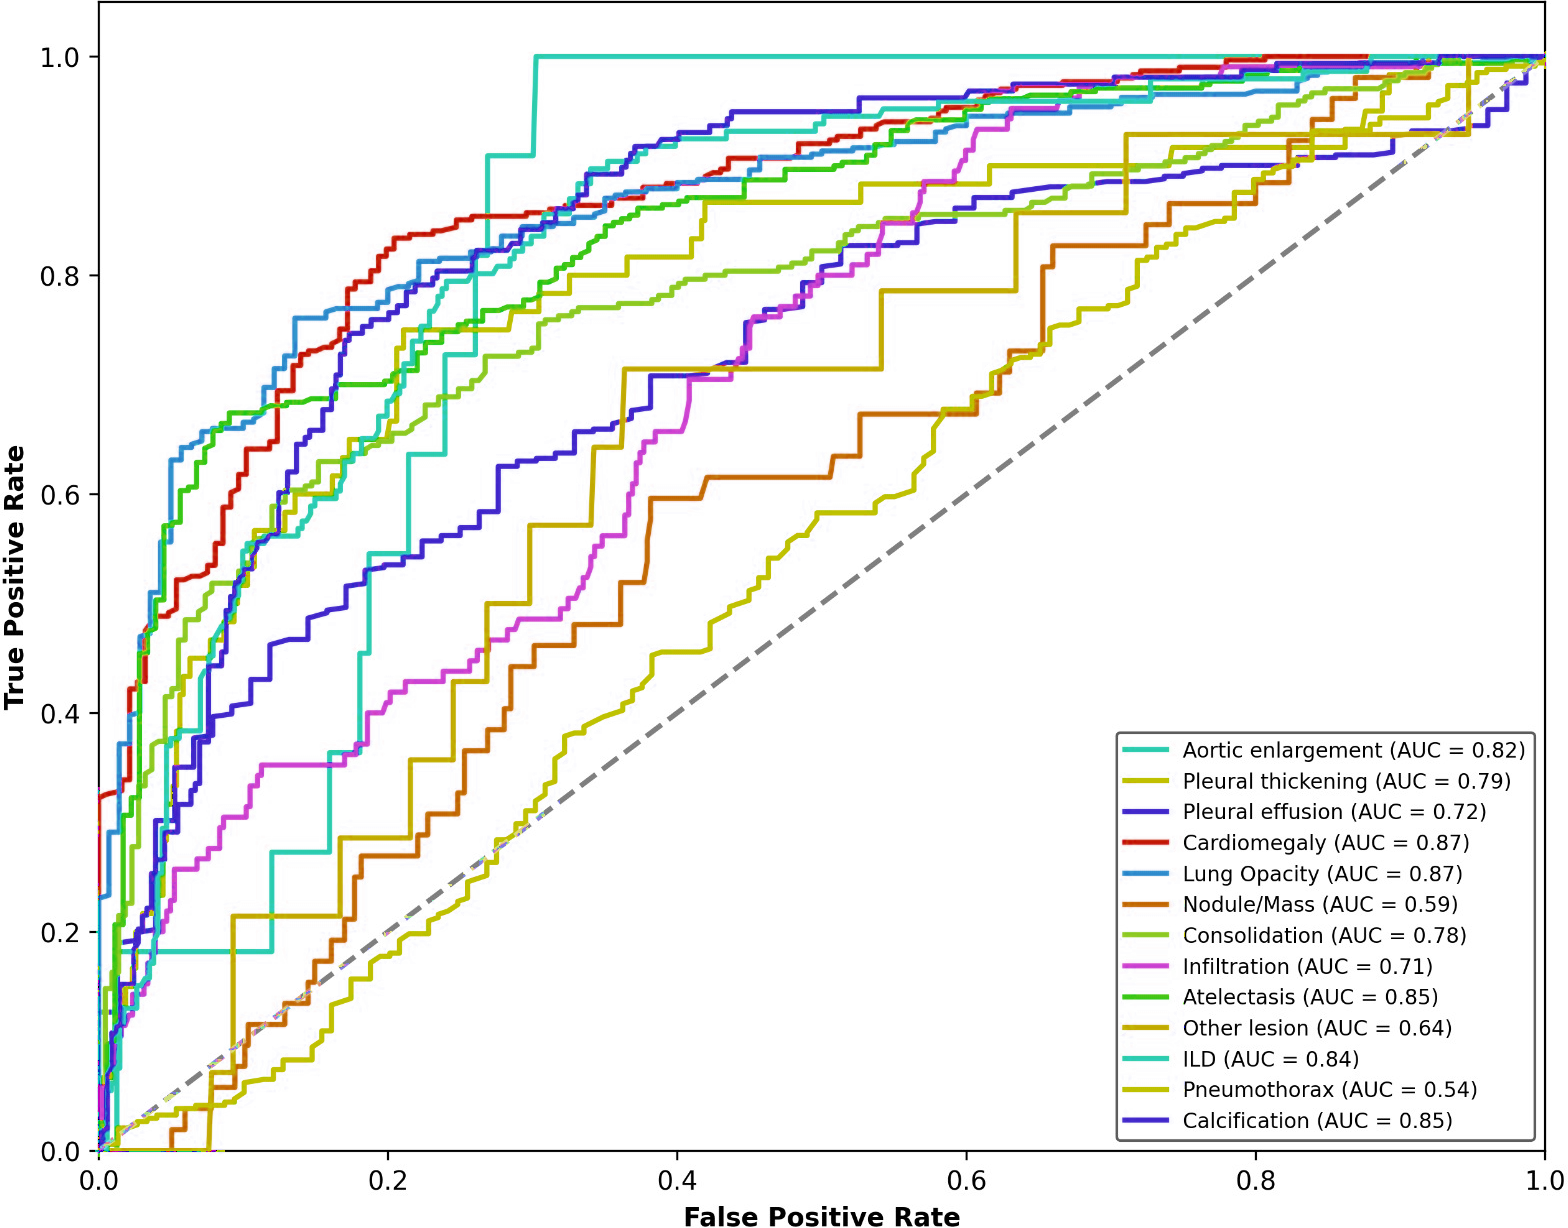
\includegraphics[width=0.85\columnwidth]{fig/roc_white.png}
\caption{Per-class ROC over the 14-category working taxonomy. Thirteen curves
are defined; Pulmonary fibrosis has no positive example.}
\label{fig:roc}
\end{figure}

\begin{figure}[!t]
\centering
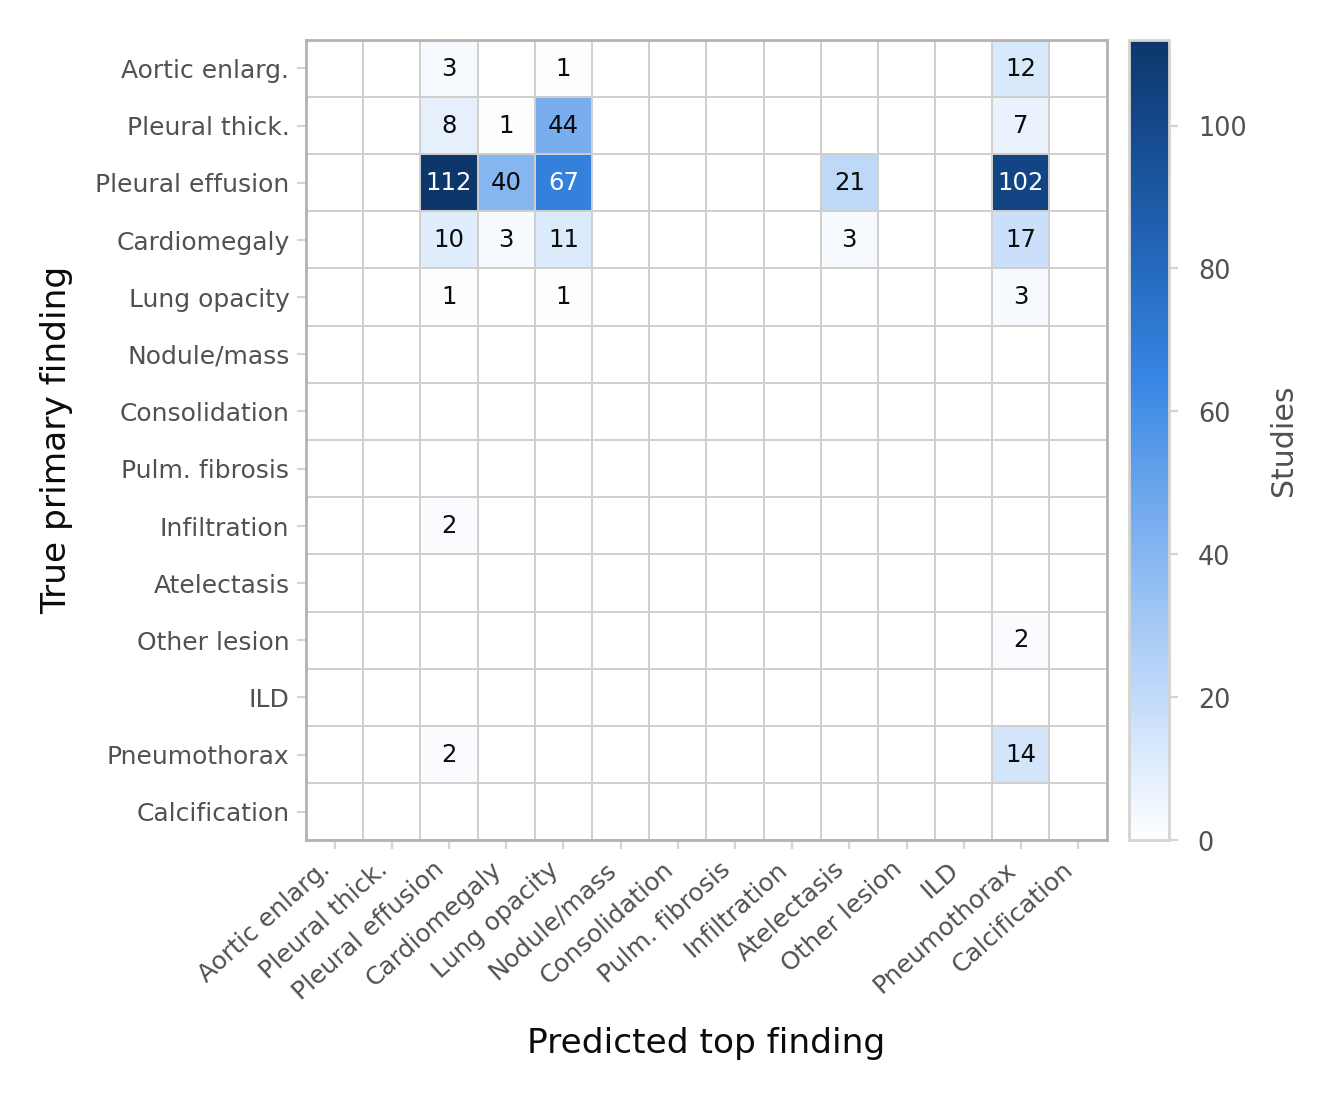
\includegraphics[width=0.96\columnwidth]{fig/cm_white.png}
\caption{True primary finding vs.\ top-ranked prediction, 487 studies. Empty
cells are zero. Predicted mass falls in five columns, and nine categories never
win.}
\label{fig:cm}
\end{figure}

The confusion matrix indicates residual prediction collapse. Fig.~\ref{fig:cm}
cross-tabulates the true primary finding against the top-ranked prediction over
487 studies with a defined primary label. Top-1 agreement is 129/487, or
26.5\%. The distribution of the predictions is more informative. Every prediction falls into one of five columns (Pleural
effusion, Cardiomegaly, Lung Opacity, Atelectasis and Pneumothorax), and nine
of the fourteen categories are never the top choice on any study. Pleural
effusion accounts for 342/487 (70\%) of the subset and is recovered 112 times,
but is assigned to Pneumothorax on 102 occasions. Concentrating confidence on a
small number of prevalent classes sustains the micro F1 while producing poor
ranking within the rare classes. This is the behaviour that the loss design
targets, and it is only partly addressed at partition scale.

The 0\% exact match ratio is expected rather than a failure, and the measured
latency supports interactive use. With $C = 14$ independent binary decisions a
fully correct output vector requires all 14 to be right at once, and published
systems on comparable vocabularies also report near-zero subset accuracy. The
metric is included because omitting it gives an overly favourable impression of
performance. Per-image inference below 25\,ms is roughly twice as fast as the
50\,ms target, leaving headroom for the Grad-CAM backward pass and rendering.

An ablation holding all other settings fixed orders the individual effects.
Removing ImageNet initialization is the most damaging single change (micro F1
$0.7528 \rightarrow 0.5940$), which is unsurprising at this scale, since without
transfer there is not enough data to learn generic edge and texture filters.
Replacing Focal Loss with BCE costs $-0.070$ ($\rightarrow 0.6828$), the direct
quantitative case for the imbalance treatment and the largest effect
attributable to a design choice made here rather than inherited. Dropping
augmentation costs $-0.042$ ($\rightarrow 0.7110$) and dropping checkpoint
averaging $-0.021$ ($\rightarrow 0.7320$). These last two are modest, but
checkpoint averaging carries no inference cost, so it is retained.

Detection metrics on VinDr-CXR (mAP@IoU 0.50, mAP@0.50:0.95, AR@100 at the 0.30
operating point) come from the COCO evaluation output. The corrective plan,
ordered by expected impact, is as follows: retrain on the full corpus rather
than partitions p13--p19, which should lift the rare-class AUCs and break the
five-column concentration seen in Fig.~\ref{fig:cm}; add temperature scaling,
since an uncalibrated score distribution is part of the reason the top-1
routing is so concentrated; and then re-run the ablation at full scale.

\begin{figure*}[!t]
\centering
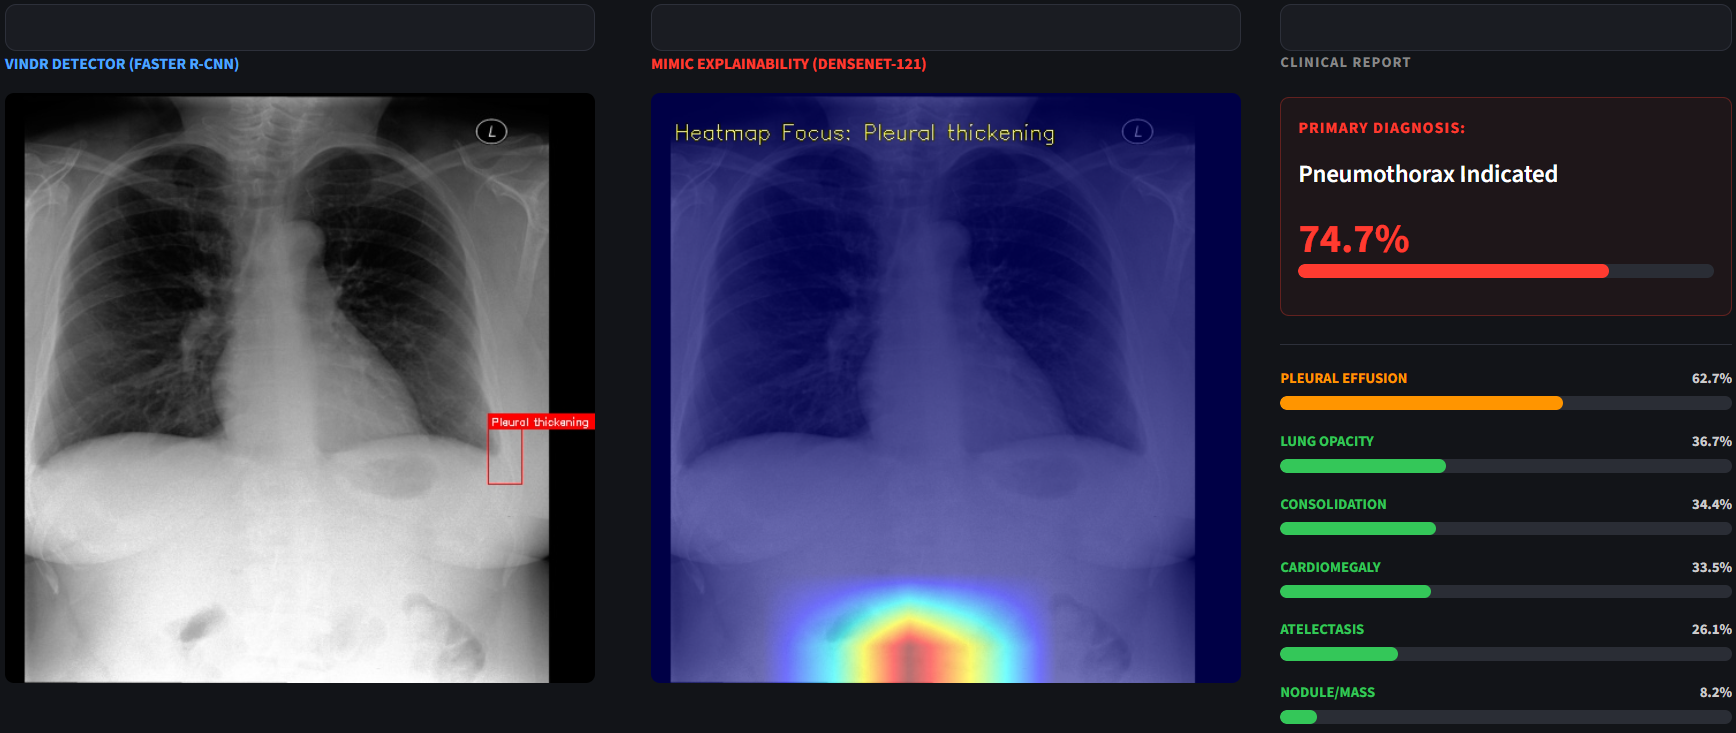
\includegraphics[width=0.75\textwidth]{fig/vis_dark.png}
\caption{The deployed MED-AI Visualizer on a deliberate failure case. The
detector localizes pleural thickening on the left lateral margin while the
classifier names pneumothorax at 74.7\%, and the saliency sits
sub-diaphragmatic rather than over the pleural margin.}
\label{fig:ui}
\end{figure*}

\section{Limitations}

Several qualifications attach to the numbers above. Training ran over patient
partitions instead of the whole corpus, which leaves the scarce pathologies
thinly represented and means the AUC quoted here should not be read as a
ceiling on what the architecture can reach. The 498-image subset gives wide confidence intervals and,
for the rarest classes, an undefined per-class AUC. No bootstrap intervals or
significance tests are reported, both of which a camera-ready version requires. MIMIC-CXR labels are NLP-derived, inherit the labeler's handling of uncertainty
and negation, and are not adjudicated ground truth
\cite{majkowska2020}. The two corpora use only partially overlapping
vocabularies, so the branches are trained separately and the unified interface
should not be read as a jointly optimized model. Downsampling to $256 \times
256$ discards detail that is material for small nodules, calcifications and
subtle pneumothorax lines, and higher resolution is a known lever
\cite{baltruschat2019}. Output probabilities are uncalibrated and should not be
read as clinical likelihoods without temperature scaling. All results are
retrospective and in-distribution, and generalization across vendors and
populations is untested. Finally, this is a research prototype with no
regulatory clearance, not evaluated in a reader study and not intended for
diagnostic use.

\section{Conclusion and Future Work}

Described here is a two-branch system for reading chest films: a
Focal-Loss-trained DenseNet-121 diagnosing over MIMIC-CXR, a Faster R-CNN/FPN
detector localizing over VinDr-CXR under radiologist supervision, and a Grad-CAM
layer and deployed viewer across both. The classification branch attains a micro F1 of 0.7528, within the
range of published DenseNet baselines, at sub-25\,ms per-image inference. The
mean AUC-ROC of 0.759 is below the published range, and two contributing
factors were identified: per-class ranking degrades to near-chance
on small focal findings, and top-1 predictions concentrate on five of fourteen
categories.

Four directions follow. The first is full-corpus retraining at higher
resolution with probability calibration, which should account for most of the
AUC gap. The second is weighted box fusion \cite{solovyev2021}
in place of greedy NMS, with transformer-based detectors evaluated alongside.
The third is joint multi-task optimization over a harmonized ontology, so that
localization supervision can regularize the classifier. The fourth is a
prospective reader study to determine whether saliency overlays alter
radiologist decisions, which would be needed to establish clinical value.

\section*{Ethics and Data Availability}

Every image used here comes from an openly distributed, de-identified,
retrospectively assembled collection; no participant was recruited
prospectively for this work. Access to MIMIC-CXR \cite{johnson2019mimic} runs
through PhysioNet under its credentialed-access terms, and its images carry
HIPAA Safe Harbor de-identification. VinDr-CXR \cite{nguyen2022} was gathered
with Institutional Review Board approval. At no point was any individual
re-identified. Trained weights and source code can be obtained from the authors
on request. We are grateful to the curators of both collections, and to the
radiologists whose reading underpins the annotations.

\begin{thebibliography}{00}
\footnotesize
\bibitem{wang2017} X. Wang \textit{et al.}, ``ChestX-ray8: Hospital-scale chest X-ray database and benchmarks on weakly-supervised classification and localization of common thorax diseases,'' in \textit{Proc. IEEE CVPR}, 2017, pp. 2097--2106.
\bibitem{rajpurkar2017} P. Rajpurkar \textit{et al.}, ``CheXNet: Radiologist-level pneumonia detection on chest X-rays with deep learning,'' \textit{arXiv:1711.05225}, 2017.
\bibitem{irvin2019} J. Irvin \textit{et al.}, ``CheXpert: A large chest radiograph dataset with uncertainty labels and expert comparison,'' in \textit{Proc. AAAI}, vol. 33, 2019, pp. 590--597.
\bibitem{johnson2019jpg} A. E. W. Johnson \textit{et al.}, ``MIMIC-CXR-JPG, a large publicly available database of labeled chest radiographs,'' \textit{arXiv:1901.07042}, 2019.
\bibitem{baltruschat2019} I. M. Baltruschat \textit{et al.}, ``Comparison of deep learning approaches for multi-label chest X-ray classification,'' \textit{Scientific Reports}, vol. 9, no. 1, p. 6381, 2019.
\bibitem{majkowska2020} A. Majkowska \textit{et al.}, ``Chest radiograph interpretation with deep learning models: Assessment with radiologist-adjudicated reference standards and population-adjusted evaluation,'' \textit{Radiology}, vol. 294, no. 2, pp. 421--431, 2020.
\bibitem{nguyen2022} H. Q. Nguyen \textit{et al.}, ``VinDr-CXR: An open dataset of chest X-rays with radiologist's annotations,'' \textit{Scientific Data}, vol. 9, no. 1, p. 429, 2022.
\bibitem{ren2015} S. Ren \textit{et al.}, ``Faster R-CNN: Towards real-time object detection with region proposal networks,'' in \textit{NeurIPS}, 2015, pp. 91--99.
\bibitem{lin2017fpn} T.-Y. Lin \textit{et al.}, ``Feature pyramid networks for object detection,'' in \textit{Proc. IEEE CVPR}, 2017, pp. 2117--2125.
\bibitem{he2016} K. He \textit{et al.}, ``Deep residual learning for image recognition,'' in \textit{Proc. IEEE CVPR}, 2016, pp. 770--778.
\bibitem{howard2019} A. Howard \textit{et al.}, ``Searching for MobileNetV3,'' in \textit{Proc. IEEE/CVF ICCV}, 2019, pp. 1314--1324.
\bibitem{solovyev2021} R. Solovyev \textit{et al.}, ``Weighted boxes fusion: Ensembling boxes from different object detection models,'' \textit{Image and Vision Computing}, vol. 107, p. 104117, 2021.
\bibitem{lin2017focal} T.-Y. Lin \textit{et al.}, ``Focal loss for dense object detection,'' in \textit{Proc. IEEE ICCV}, 2017, pp. 2980--2988.
\bibitem{selvaraju2017} R. R. Selvaraju \textit{et al.}, ``Grad-CAM: Visual explanations from deep networks via gradient-based localization,'' in \textit{Proc. IEEE ICCV}, 2017, pp. 618--626.
\bibitem{johnson2019mimic} A. E. W. Johnson \textit{et al.}, ``MIMIC-CXR, a de-identified publicly available database of chest radiographs with free-text reports,'' \textit{Scientific Data}, vol. 6, no. 1, p. 317, 2019.
\bibitem{huang2017} G. Huang \textit{et al.}, ``Densely connected convolutional networks,'' in \textit{Proc. IEEE CVPR}, 2017, pp. 4700--4708.
\bibitem{deng2009} J. Deng \textit{et al.}, ``ImageNet: A large-scale hierarchical image database,'' in \textit{Proc. IEEE CVPR}, 2009, pp. 248--255.
\bibitem{izmailov2018} P. Izmailov \textit{et al.}, ``Averaging weights leads to wider optima and better generalization,'' in \textit{Proc. UAI}, 2018, pp. 876--885.
\bibitem{micikevicius2018} P. Micikevicius \textit{et al.}, ``Mixed precision training,'' in \textit{Proc. ICLR}, 2018.
\end{thebibliography}

\end{document}
